\section{数据管理}
超级计算机架构师经常感叹需要“喂养野兽”。 
“喂养野兽”一词指的是当我们使用大量并行性时我们创建的计算机的“野兽”,并向其提供数据成为需要解决的关键挑战。

在异构机器上提供 SYCL 程序需要小心,以确保数据在需要时位于需要的位置。 
在大型程序中,这可能需要大量工作。 在现有的 C++ 程序中,仅仅弄清楚如何管理所需的所有数据移动就可能是一场噩梦。

我们将仔细解释管理数据的两种方式:统一共享内存(USM)和Buffer。 
USM 是基于指针的,C++ 程序员对此很熟悉。 Buffer提供了更高级别的抽象。 有选择是好的。

我们需要控制数据的移动,本章将介绍实现这一目标的选项。

在第 2 章中,我们研究了如何控制代码的执行位置。 我们的代码需要数据作为输入并生成数据作为输出。 
由于我们的代码可能在多个设备上运行,并且这些设备不一定共享内存,因此我们需要管理数据移动。 
即使数据是共享的(例如使用 USM),同步和一致性也是我们需要理解和管理的概念。

一个合乎逻辑的问题可能是“为什么编译器不自动为我们完成所有事情?” 虽然可以自动为我们处理很多事情,
但如果我们不宣称自己是程序员,那么性能通常不是最佳的。 
在实践中,为了获得最佳性能,我们在编写异构程序时需要关注代码放置(第 2 章)和数据移动(本章)。

本章概述了管理数据,包括控制数据使用的顺序。 它是对前一章的补充,前一章向我们展示了如何控制代码的运行位置。 
本章帮助我们有效地使数据出现在我们要求代码运行的位置,这不仅对于正确执行应用程序很重要,
而且对于最大限度地减少执行时间和功耗也很重要。


\subsection{介绍}
没有数据,计算就毫无意义。 加速计算的全部目的是更快地产生答案。 
这意味着数据并行计算最重要的方面之一是它们如何访问数据,并将加速器设备引入机器使情况进一步复杂化。 
在传统的基于单插槽 CPU 的系统中,我们只有一个内存。 加速器设备通常有自己的附加存储器,无法从主机直接访问。 
因此,支持分立设备的并行编程模型必须提供管理这些多个存储器并在它们之间移动数据的机制。

在本章中,我们概述了数据管理的各种机制。 
我们介绍了统一共享内存和数据管理的Buffer抽象,并描述了Kernel执行和数据移动之间的关系。

\subsection{数据管理问题}
从历史上看,用于并行编程的共享内存模型的优点之一是它们提供了单一的共享内存视图。 拥有这种单一的内存视图可以简化生活。 
我们不需要做任何特殊的事情来从并行任务访问内存(除了适当的同步以避免数据竞争)。 
虽然某些类型的加速器设备(例如集成 GPU)与主机 CPU 共享内存,但许多离散加速器都有自己的本地内存,
与 CPU 的内存分开,如图 3-1 所示。

\begin{figure}[H]
	\centering
	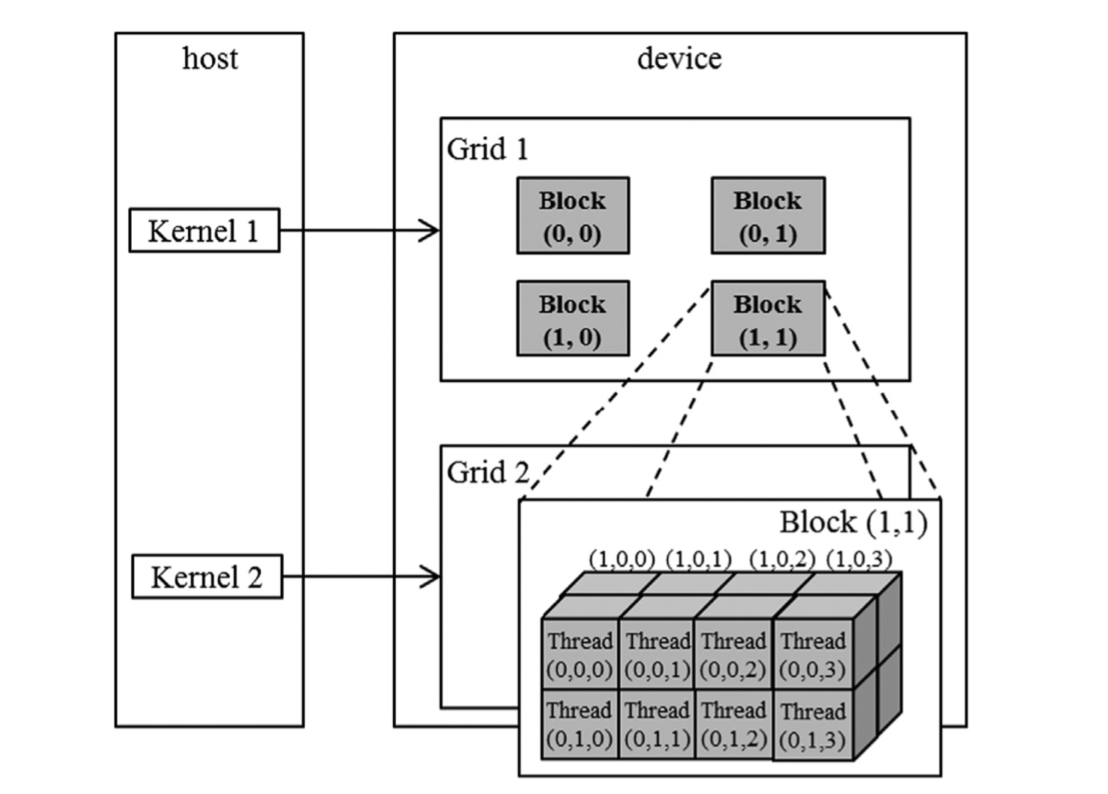
\includegraphics[width=0.9\textwidth]{figs/F3.1.png}
	\caption{\textit{多个离散存储器}}
\end{figure}

\subsection{本地设备与远程设备}
在使用直接连接到设备的内存(而不是远程内存)读取和写入数据时,在设备上运行的程序通常性能更好。 
我们将对直接连接的存储器的访问称为本地访问。 对另一台设备内存的访问是远程访问。 
远程访问往往比本地访问慢,因为它们必须通过带宽较低和/或延迟较高的数据链路进行传输。 
这意味着将计算和它将使用的数据放在一起通常是有利的。 
为了实现这一目标,我们必须以某种方式确保数据在不同内存之间复制或迁移,以便将其移至更靠近计算发生的位置。

\subsection{管理多个内存}
管理多个内存大致可以通过两种方式完成:显式地通过我们的程序或隐式地通过 SYCL 运行时库。 
每种方法都有其优点和缺点,我们可以根据情况或个人喜好选择其中一种。

\subsubsection{显式数据移动}
\begin{figure}[H]
	\centering
	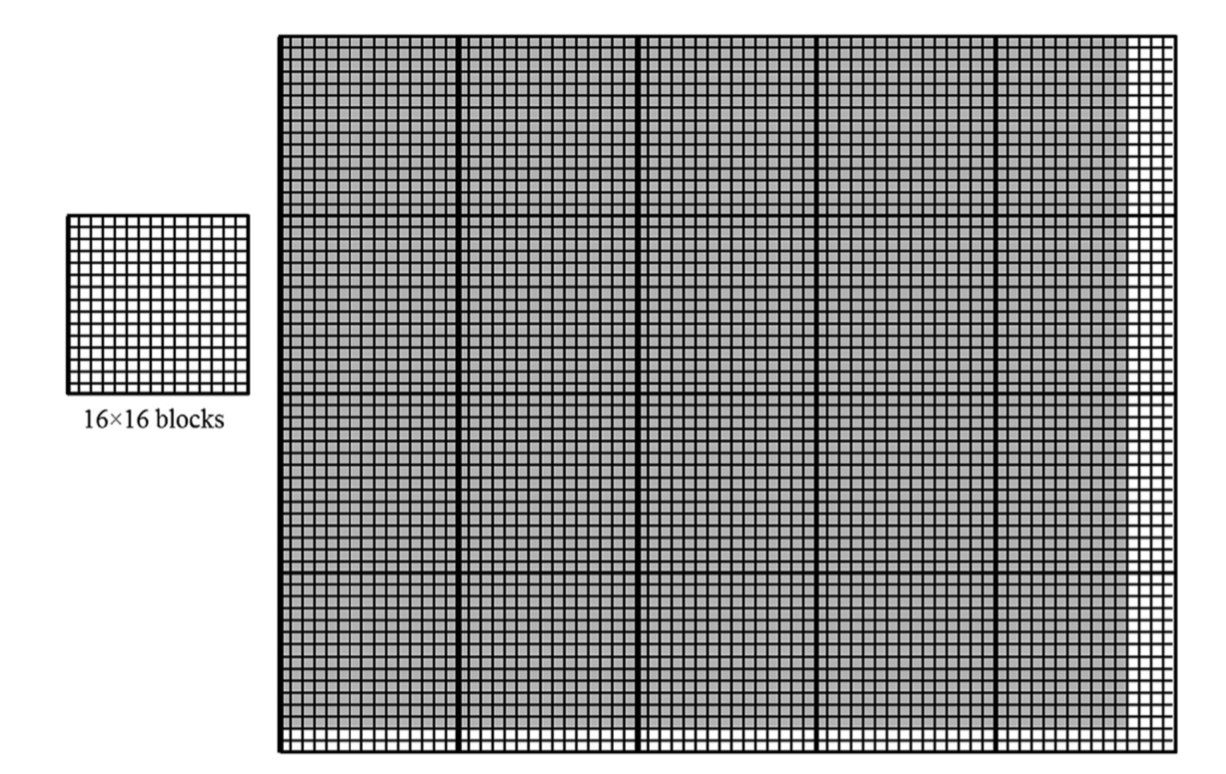
\includegraphics[width=0.9\textwidth]{figs/F3.2.png}
	\caption{\textit{数据移动和Kernel执行}}
\end{figure}

管理多个存储器的一种选择是在不同存储器之间显式复制数据。 
图 3-2 显示了一个具有离散加速器的系统,我们必须首先将Kernel所需的任何数据从主机内存复制到加速器内存。 
Kernel计算结果后,我们必须将这些结果复制回主机,然后主机程序才能使用该数据。

显式数据移动的主要优点是我们可以完全控制数据在不同内存之间传输的时间。 
这很重要,因为重叠计算与数据传输对于在某些硬件上获得最佳性能至关重要。

显式数据移动的缺点是指定所有数据移动可能很乏味且容易出错。 
传输不正确的数据量或不确保在Kernel开始计算之前已传输所有数据可能会导致不正确的结果。 
从一开始就确保所有数据移动正确可能是一项非常耗时的任务。

\subsubsection{隐式数据}
程序控制的显式数据移动的替代方案是由并行运行时或驱动程序控制的隐式数据移动。 
在这种情况下,并行运行时不需要在不同内存之间进行显式复制,而是负责确保数据在使用之前传输到适当的内存。

隐式数据移动的优点是,应用程序无需花费太多精力即可利用直接连接到设备的更快内存。 
所有繁重的工作都是由运行时自动完成的。 
这也减少了在程序中引入错误的机会,因为运行时将自动识别何时必须执行数据传输以及必须传输多少数据。

隐式数据移动的缺点是我们对运行时隐式机制的行为控制较少或无法控制。 
运行时将提供功能正确性,但可能无法以最佳方式移动数据,以确保计算与数据传输的最大重叠,这可能会对程序性能产生负面影响。

\subsubsection{选择正确的策略}
为项目选择最佳策略可能取决于许多不同的因素。 不同的策略可能适合程序开发的不同阶段。 
我们甚至可以决定最好的解决方案是混合和匹配程序不同部分的显式和隐式方法。 
我们可能会选择开始使用隐式数据移动来简化将应用程序移植到新设备的过程。 
当我们开始调整应用程序的性能时,我们可能会开始在代码的性能关键部分用显式数据移动替换隐式数据移动。 
未来的章节将介绍如何将数据传输与计算重叠以优化性能。

\subsection{USM、Buffer 和 Images}
管理内存有三个抽象:统一共享内存(USM)、Buffer 和 Images。 USM 是一种基于指针的方法,C/C++ 程序员应该熟悉。 
USM 的优点之一是更容易与现有的操作指针的 C++ 代码集成。 Buffer(由Buffer模板类表示)描述一维、二维或三维数组。 
它们提供了可以在主机或设备上访问的内存的抽象视图。 Buffer不由程序直接访问,而是通过访问器对象使用。 
Images充当一种特殊类型的Buffer,提供特定于Images处理的额外功能。 
此功能包括对特殊Images格式的支持、使用采样器对象读取Images等等。 
Buffer和Images是强大的抽象,可以解决许多问题,但重写现有代码中的所有接口以接受Buffer或访问器可能非常耗时。 
由于Buffer和Images的接口基本相同,因此本章的其余部分将仅关注 USM 和Buffer。

\subsection{统一共享内存}
USM 是我们可用于数据管理的一种工具。 
USM 是一种基于指针的方法,使用 malloc 或 new 分配数据的 C 和 C++ 程序员应该熟悉它。 
USM 简化了移植大量使用指针的现有 C/C++ 代码的过程。 支持USM的设备支持统一的虚拟地址空间。 
拥有统一的虚拟地址空间意味着主机上的 USM 分配例程返回的任何指针值都将是设备上的有效指针值。 
我们不必手动转换主机指针来获取“设备版本”——我们在主机和设备上看到相同的指针值。

USM 的更详细描述可以在第 6 章中找到。

\subsubsection{通过指针访问内存}
\begin{figure}[H]
	\centering
	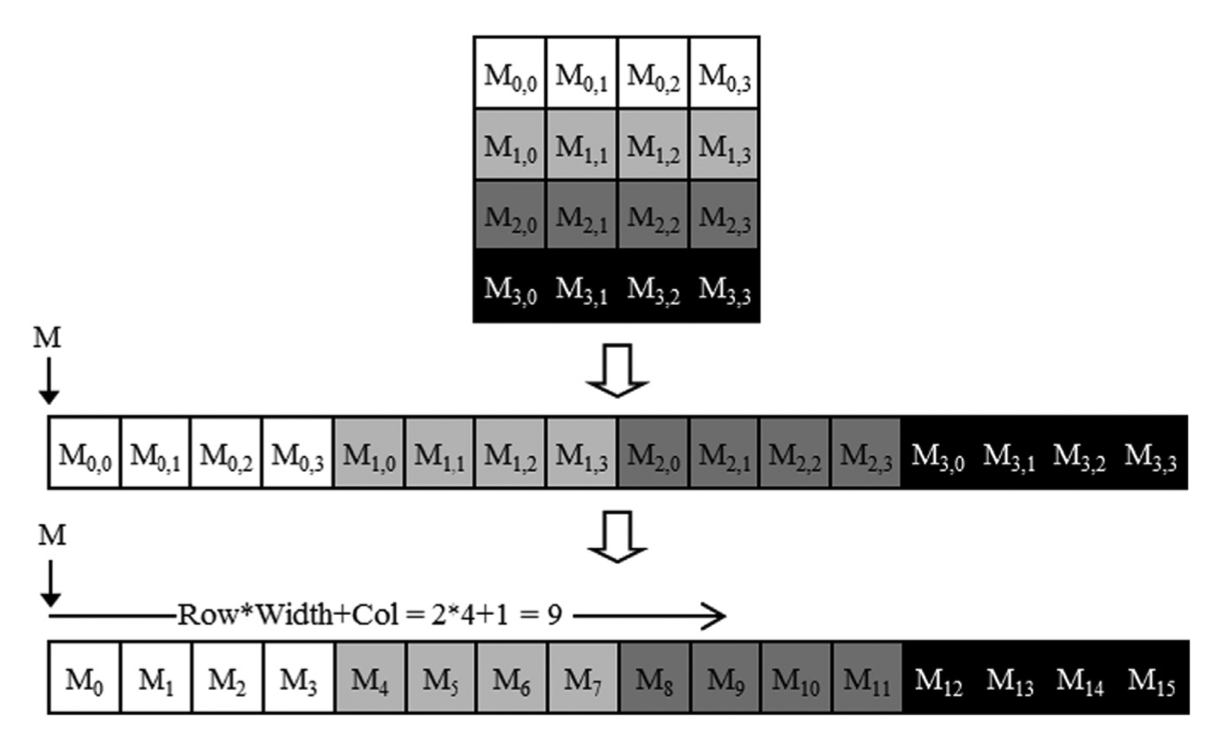
\includegraphics[width=0.9\textwidth]{figs/F3.3.png}
	\caption{\textit{USM allocation types}}
\end{figure}

由于当系统同时包含主机内存和一定数量的设备连接本地内存时,并非所有内存都是平等创建的,
因此 USM 定义了三种不同类型的分配:设备、主机和共享。 所有类型的分配都在主机上执行。 
图 3-3 总结了每种分配类型的特征。

设备分配发生在设备附加内存中。 这样的分配可以在设备上读取和写入,但不能从主机直接访问。 
我们必须使用显式复制操作在主机内存中的常规分配和设备分配之间移动数据。

主机分配发生在主机内存中,主机和设备上都可以访问该内存。 这意味着相同的指针值在主机代码和设备Kernel中都有效。 
然而,当访问这样的指针时,数据总是来自主机存储器。 如果在设备上访问,数据不会从主机迁移到设备本地内存。 
相反,数据通常通过总线发送,例如将设备连接到主机的 PCI Express (PCI-E)。

主机和设备上都可以访问共享分配。 在这方面,它与主机分配非常相似,
但不同之处在于数据现在可以在主机内存和设备本地内存之间迁移。 
这意味着迁移发生后,设备上的访问将从更快的设备本地内存中进行,而不是通过延迟较高的连接远程访问主机内存。 
通常,这是通过运行时内部的机制和对我们隐藏的较低级别驱动程序来完成的。

\subsubsection{USM 和数据移动}
USM 支持显式和隐式数据移动策略,不同的分配类型映射到不同的策略。 
设备分配要求我们在主机和设备之间显式移动数据,而主机和共享分配提供隐式数据移动。

\paragraph{USM 中的显式数据移动}

USM 的显式数据移动是通过设备分配以及队列和 Handler 类中的特殊 memcpy() 来完成的。 
我们将 memcpy() 操作(动作)排入队列,以将数据从主机传输到设备或从设备传输到主机。

\begin{figure}[H]
	\centering
	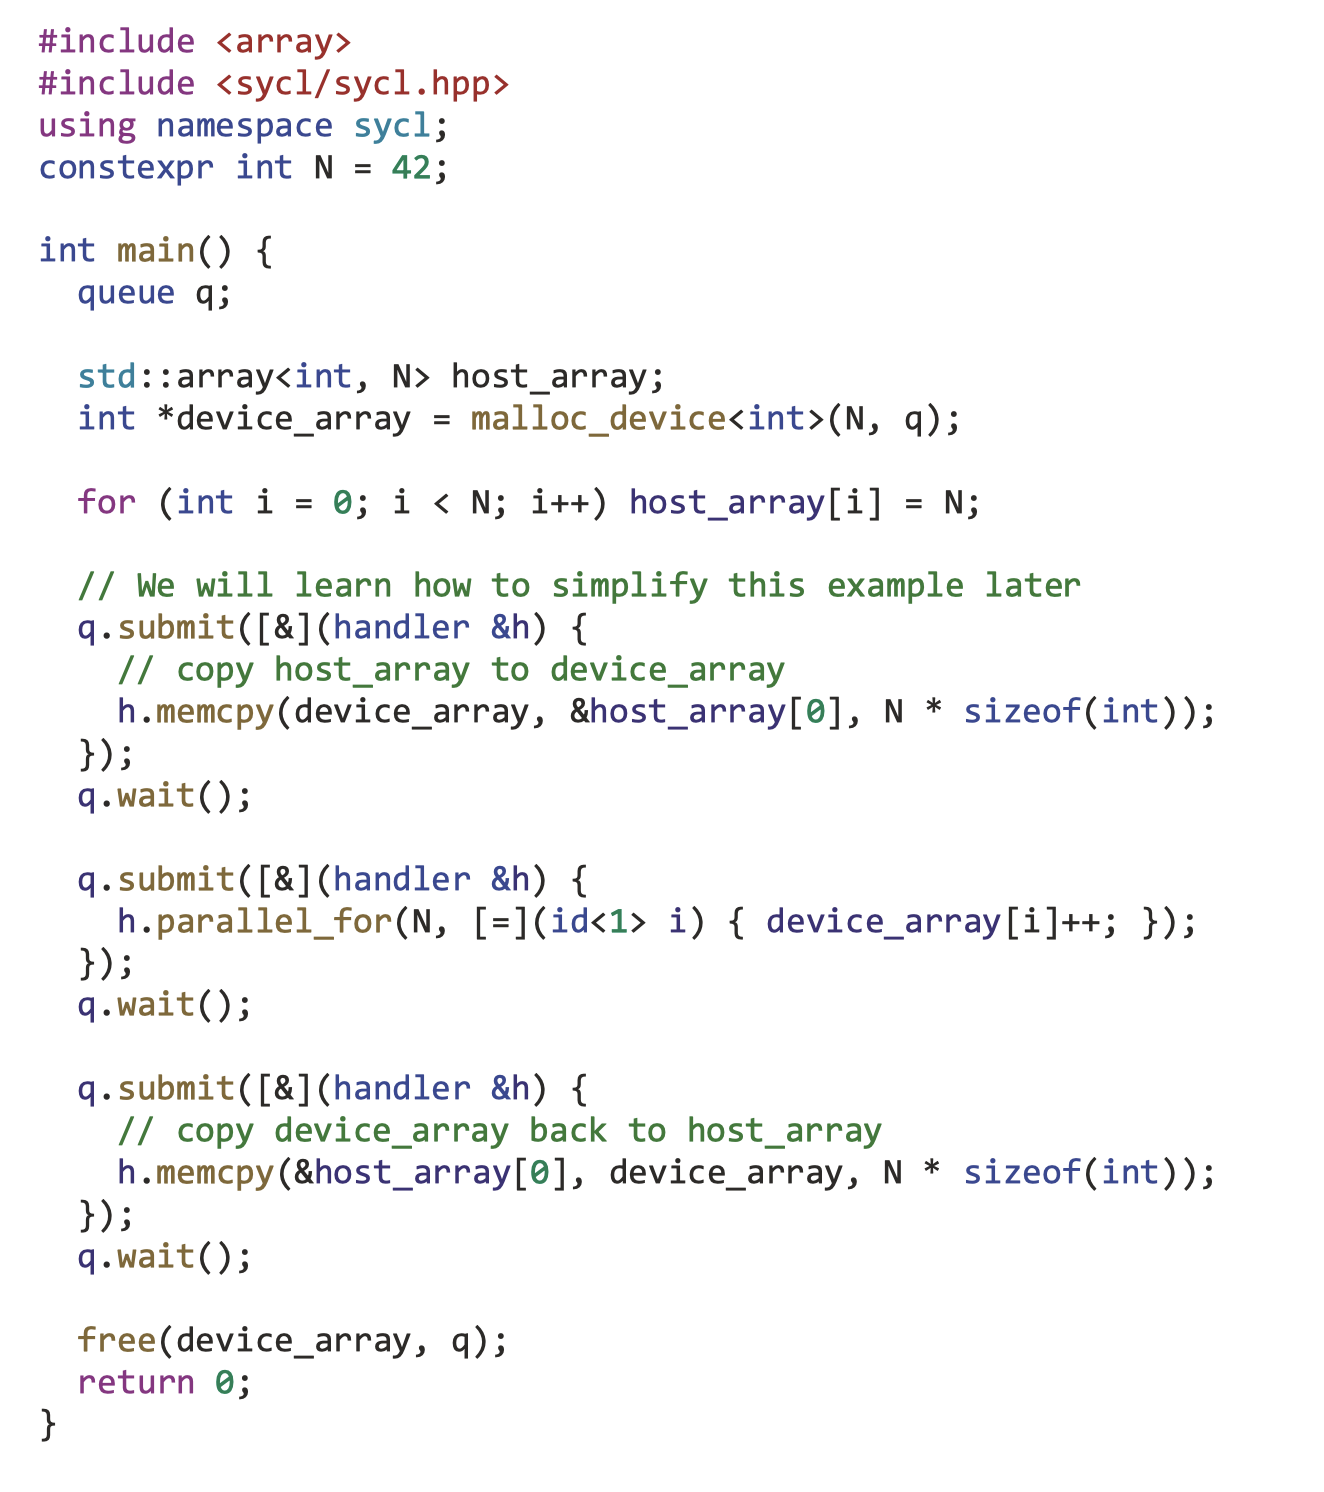
\includegraphics[width=0.9\textwidth]{figs/F3.4.png}
	\caption{\textit{USM explicit data movement}}
\end{figure}

图 3-4 包含一个在设备分配上运行的Kernel。 在Kernel使用 memcpy() 操作执行之前和之后,
数据会在 host\_array 和 device\_array 之间复制。 
调用队列上的 wait() 可确保在Kernel执行之前完成到设备的复制,并确保在数据复制回主机之前Kernel已完成。 
我们将在本章后面学习如何消除这些调用。

\paragraph{USM 中的隐式数据移动}

USM 的隐式数据移动是通过主机和共享分配来完成的。 
通过这些类型的分配,我们不需要显式插入复制操作来在主机和设备之间移动数据。 
相反,我们只需访问Kernel内部的指针,任何所需的数据移动都会自动执行,无需程序员干预(只要您的设备支持这些分配)。 
这极大地简化了现有代码的移植:最多我们只需要简单地用适当的 USM 分配函数(以及调用 free 来释放内存)
替换任何 malloc 或 new ,并且一切都应该正常工作。

\begin{figure}[H]
	\centering
	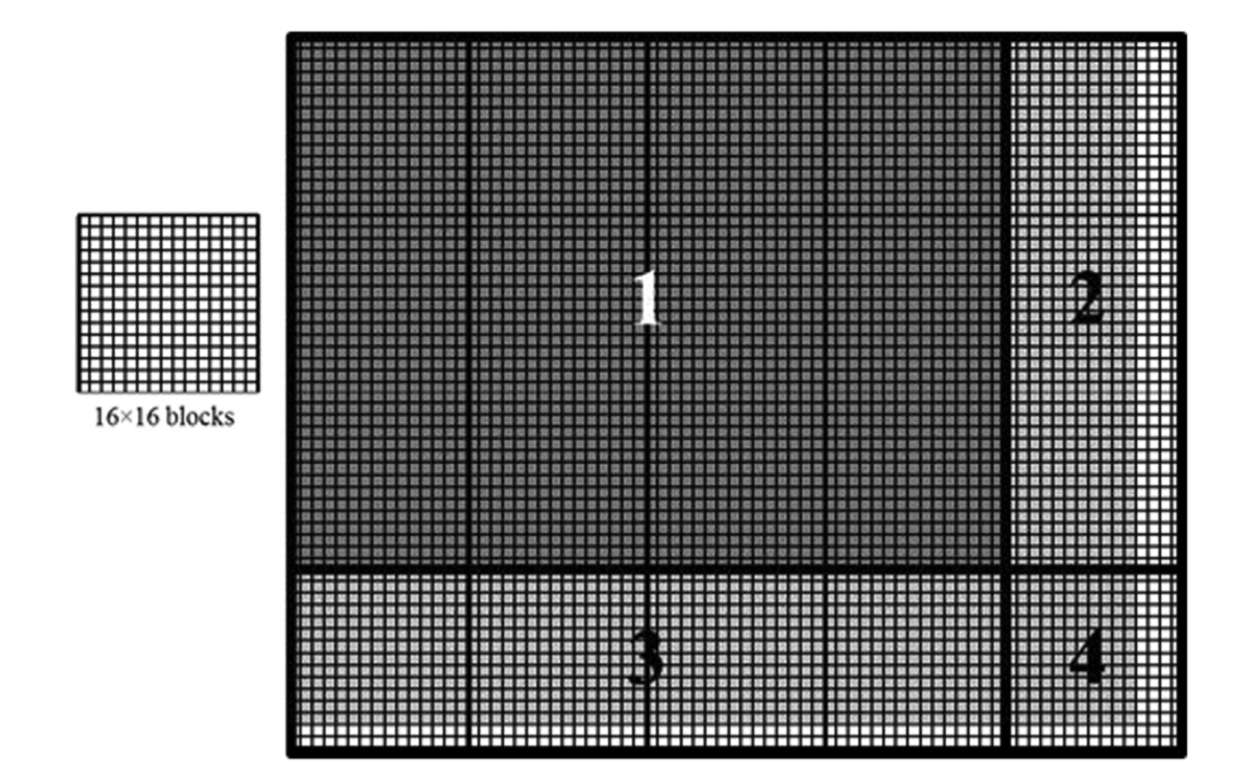
\includegraphics[width=0.9\textwidth]{figs/F3.5.png}
	\caption{\textit{USM implicit data movement}}
\end{figure}

在图 3-5 中,我们创建了两个数组:host\_array 和 shared\_array,分别是主机分配和共享分配。 
虽然主机和共享分配都可以在主机代码中直接访问,但我们在这里只初始化 host\_array 。 
同样,可以在Kernel内部直接访问,进行数据的远程读取。 
运行时确保shared\_array在Kernel访问它之前在设备上可用,并且当主机代码稍后读取它时将其移回,所有这些都无需程序员干预。

\subsection{Buffer}
为数据管理提供的另一个抽象是 Buffer 对象。 Buffer 是一种数据抽象,表示给定 C++ 类型的一个或多个对象。 
Buffer对象的元素可以是标量数据类型(例如 int、float 或 double)、向量数据类型(第 11 章)或用户定义的类或结构。 
SYCL 2020 定义了一个新概念“设备可复制”,它扩展了可简单复制的概念,并添加了允许类型集。 
特别是,如果常见 C++ 类(例如 std::array、std::pair、std::tuple 或 std::span)中的模板化类型本身是设备可复制的,
那么使用这些类型构建的那些 C++ 类特化也是设备可复制的。 
在将数据类型与Buffer一起使用之前,请注意您的数据类型是设备可复制的!

虽然Buffer本身是单个对象,但Buffer封装的 C++ 类型可以是包含多个对象的数组。 
Buffer代表数据对象而不是特定的内存地址,因此不能像常规 C++ 数组一样直接访问。 
事实上,出于性能原因,Buffer对象可能映射到多个不同设备上的多个不同内存位置,甚至映射到同一设备上。 
相反,我们使用访问器对象来读取和写入Buffer。

Buffer的更详细描述可以在第 7 章中找到。

\subsubsection{创建Buffer}
可以通过多种方式创建Buffer。 最简单的方法是简单地构造一个新的Buffer,其范围指定Buffer的大小。 
然而,以这种方式创建Buffer并不会初始化其数据,这意味着我们必须首先通过其他方式初始化Buffer,
然后才能尝试从中读取有用的数据。

还可以根据主机上的现有数据创建Buffer。 
这是通过调用几个构造函数之一来完成的,这些构造函数采用指向现有主机分配的指针、
一组 InputIterators 或具有某些属性的容器。 在Buffer构造期间,数据从现有主机分配复制到Buffer对象的主机内存中。 
还可以使用 SYCL 互操作性功能(例如,从 OpenCL cl\_mem 对象)从特定于后端的对象创建Buffer。 
有关如何执行此操作的更多详细信息,请参阅有关互操作性的章节。

\subsubsection{访问Buffer}
主机和设备可能无法直接访问Buffer(除非通过此处未描述的高级且不常用的机制)。 
相反,我们必须创建访问器才能读取和写入Buffer。 
访问器为运行时提供有关我们计划如何使用Buffer中的数据的信息,使其能够正确安排数据移动。

\subsubsection{访问模式}
\begin{figure}[H]
	\centering
	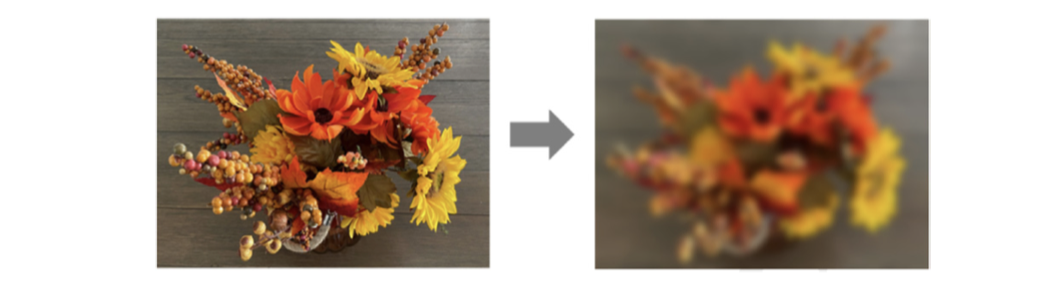
\includegraphics[width=0.9\textwidth]{figs/F3.6.png}
	\caption{\textit{Buffer and accessors}}
\end{figure}

\begin{figure}[H]
	\centering
	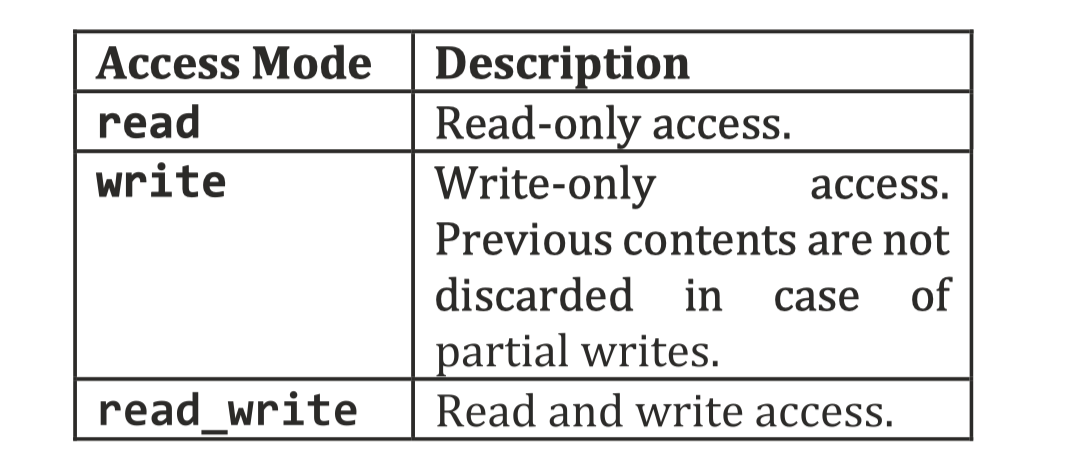
\includegraphics[width=0.9\textwidth]{figs/F3.7.png}
	\caption{\textit{Buffer access modes}}
\end{figure}

创建访问器时,我们可以通知运行时我们将如何使用它来提供更多优化信息。 我们通过指定访问模式来做到这一点。 
访问模式在图 3-7 中描述的 access\_mode 枚举类中定义。 
在图 3-6 所示的代码示例中,访问器 my\_accessor 是使用默认访问模式 access\_mode::read\_write 创建的。 
这让运行时知道我们打算通过 my\_accessor 读取和写入Buffer。 访问模式是运行时优化隐式数据移动的方式。 
例如,access\_mode::read 告诉运行时,在该Kernel开始执行之前,数据需要在设备上可用。 
如果Kernel仅通过访问器读取数据,则无需在Kernel完成后将数据复制回主机,因为我们没有修改它。 
同样,access\_mode::write 让运行时知道我们将修改Buffer的内容,并且可能需要在计算结束后将结果复制回来。

使用正确的模式创建访问器可以为运行时提供有关如何在程序中使用数据的更多信息。 
运行时使用访问器来排序数据的使用,但它也可以使用此数据来优化Kernel的调度和数据移动。 
第 7 章更详细地描述了访问模式和优化标签。

\subsection{对数据的使用进行排序}
Kernel可以被视为提交执行的异步任务。 这些任务必须提交到队列,并安排它们在设备上执行。 
在许多情况下,Kernel必须按特定顺序执行,以便计算出正确的结果。 
如果要获得正确结果需要任务 A 先于任务 B 执行,则称任务 A 和任务 B 之间存在依赖关系。
\footnote{请注意,您可能会看到“dependence”和“dependences”有时在其他文本中拼写为“dependency”和“dependencies”。
它们的意思是一样的,但我们倾向于在几篇关于数据流分析的重要论文中使用的拼写。
请参阅 https://dl.acm.org/doi/pdf/10.1145/75277.75280 
和 https:// dl.acm.org/doi/pdf/10.1145/113446.113449。}

然而,Kernel并不是必须调度的唯一任务形式。 在Kernel开始执行之前,Kernel访问的任何数据都需要在设备上可用。 
这些数据依赖性可以以从一个设备到另一设备的数据传输的形式创建额外的任务。 
数据传输任务可以是显式编码的复制操作或更常见的由运行时执行的隐式数据移动。

如果我们获取程序中的所有任务以及它们之间存在的依赖关系,我们可以使用它来将信息可视化为图表。 
该任务图具体来说是有向无环图(DAG),其中节点是任务,边是依赖关系。 
该图是有向的,因为依赖关系是单向的:任务 A 必须在任务 B 之前发生。该图是非循环的,
因为它不能包含从节点返回到自身的任何循环或路径。

\begin{figure}[H]
	\centering
	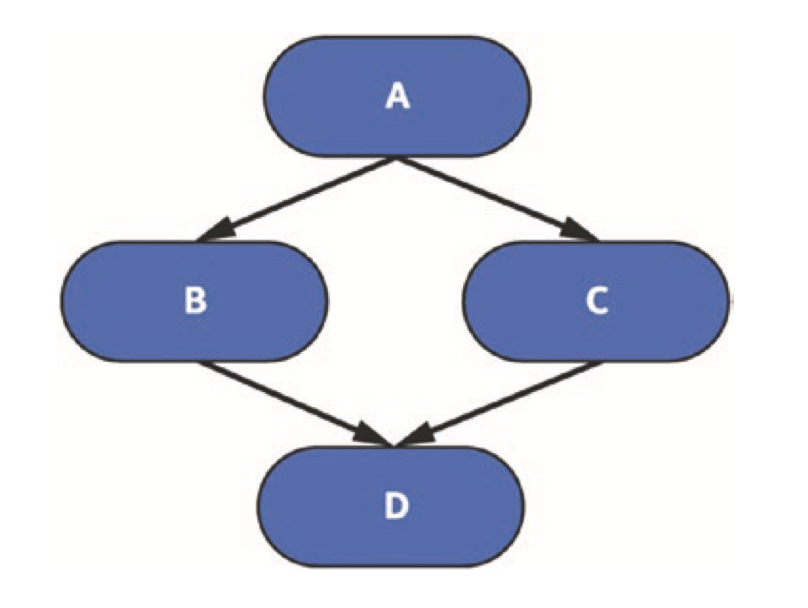
\includegraphics[width=0.9\textwidth]{figs/F3.8.png}
	\caption{\textit{简单的任务图}}
\end{figure}

在图 3-8 中,任务 A 必须在任务 B 和 C 之前执行。同样,B 和 C 必须在任务 D 之前执行。
由于 B 和 C 之间没有依赖关系,因此运行时可以自由地以任何顺序执行它们 (甚至并行)只要任务 A 已经执行。 
因此,该图可能的合法顺序是 A $\rightarrow$ B $\rightarrow$ C $\rightarrow$ D、
A $\rightarrow$ C $\rightarrow$ B $\rightarrow$ D,如果 B 和 C 可以同时执行,
甚至是 A $\rightarrow$ \{B,C\} $\rightarrow$ D。

\begin{figure}[H]
	\centering
	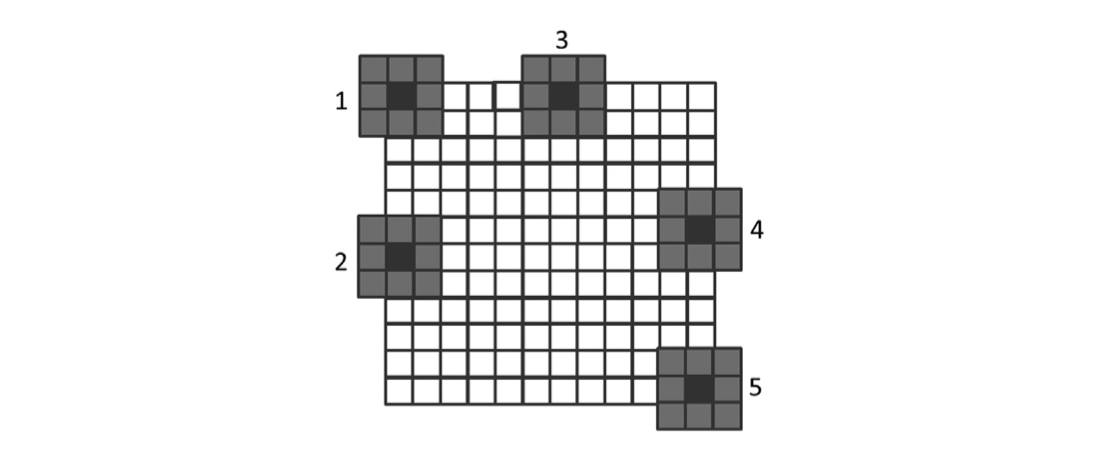
\includegraphics[width=0.9\textwidth]{figs/F3.9.png}
	\caption{\textit{具有不相交依赖关系的任务图}}
\end{figure}

任务可能与所有任务的子集具有依赖性。 在这些情况下,我们只想指定对正确性重要的依赖关系。 
这种灵活性为运行时提供了优化任务图执行顺序的自由度。 
在图 3-9 中,我们扩展了图 3-8 中的早期任务图,添加了任务 E 和 F,其中 E 必须在 F 之前执行。
但是,任务 E 和 F 与节点 A、B、C 和 D 没有依赖关系。 这允许运行时从许多可能的合法顺序中进行选择来执行所有任务。

有两种不同的方法来对队列中任务的执行(例如启动Kernel)进行建模:队列可以按照提交的顺序执行任务,
也可以按照我们指定的任何依赖项的任何顺序执行任务。 我们可以通过多种机制来定义正确排序所需的依赖关系。

\subsubsection{有序队列}
\begin{figure}[H]
	\centering
	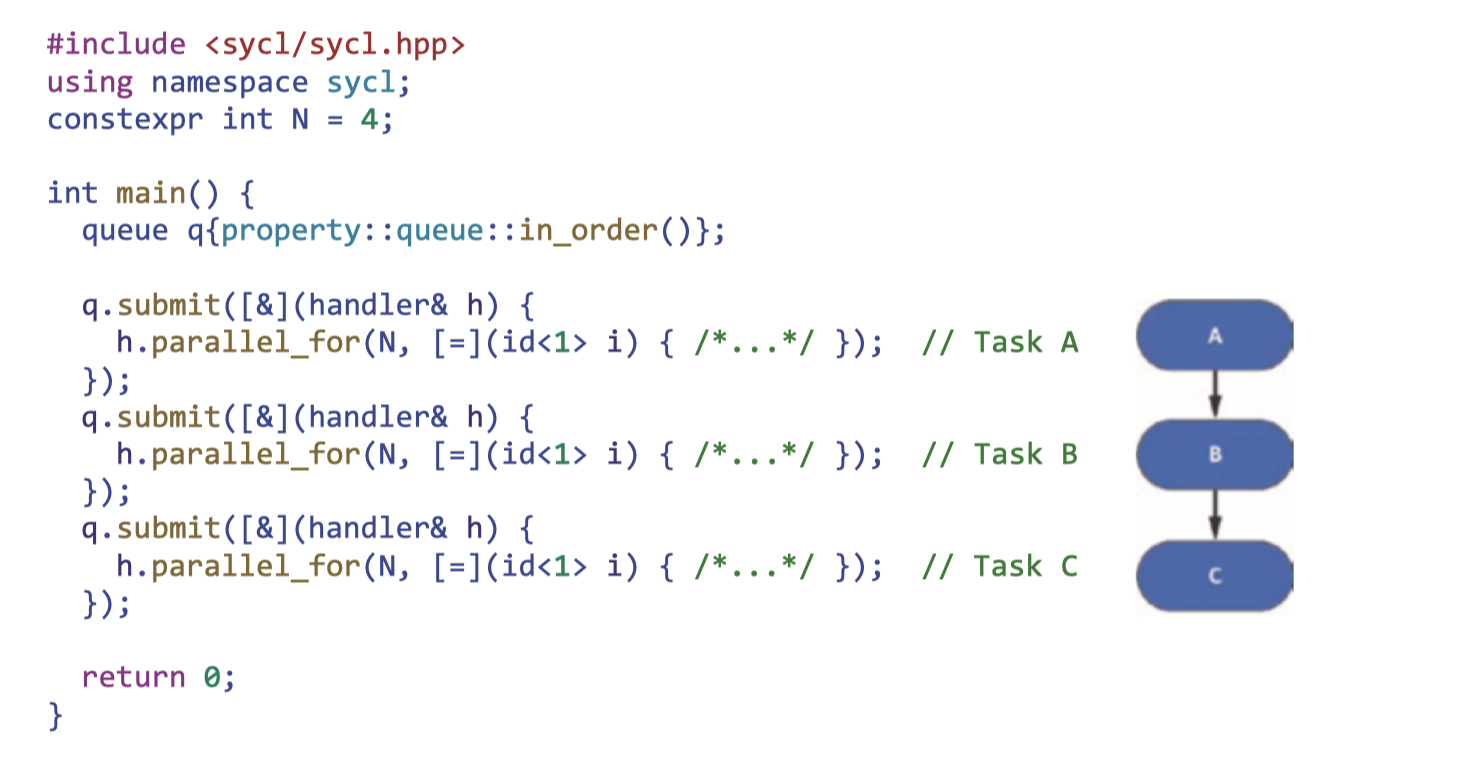
\includegraphics[width=0.9\textwidth]{figs/F3.10.png}
	\caption{\textit{In-order queue usage}}
\end{figure}

对任务进行排序的最简单选项是将它们提交到有序队列对象。 有序队列按照任务提交的顺序执行任务,如图 3-10 所示。 
它们直观的任务排序意味着有序队列具有简单性的优点,但具有序列化任务的缺点,即使独立任务之间不存在依赖性。 
有序队列在启动应用程序时非常有用,因为它们简单、直观、执行顺序确定,并且适合许多代码。

\subsubsection{无序队列}
由于队列对象是无序队列(除非使用 inorder 队列属性创建),因此它们必须提供对提交给它们的任务进行排序的方法。 
队列通过让我们通知运行时任务之间的依赖关系来对任务进行排序。 可以使用命令组显式或隐式地指定这些依赖性。 
我们将在以下部分中分别考虑它们。

命令组是指定任务及其依赖性的对象。 命令组通常编写为 C++ lambda 表达式,作为参数传递给队列对象的 Submit() 方法。 
该 lambda 的唯一参数是对Handler对象的引用。 Handler对象在命令组内部使用来指定操作、创建访问器并指定依赖关系。

\paragraph{与事件的显式依赖关系}

任务之间的显式依赖关系类似于我们看到的示例(图 3-8),其中任务 A 必须在任务 B 之前执行。
以这种方式表达依赖关系侧重于基于发生的计算而不是计算访问的数据的显式排序 。 
请注意,表达计算之间的依赖关系主要与使用 USM 的代码相关,因为使用Buffer的代码通过访问器表达大多数依赖关系。 
在图 3-4 和 3-5 中,我们只是告诉队列等待所有先前提交的任务完成,然后再继续。 
相反,我们可以通过事件对象来表达任务依赖性。 将命令组提交到队列时,submit() 方法返回一个事件对象。 
这些事件可以通过两种方式使用。

首先,我们可以通过显式调用事件的 wait() 方法来通过主机进行同步。 
这会强制运行时等待生成事件的任务完成执行,然后主机程序才能继续执行。 
显式等待事件对于调试应用程序非常有用,但 wait() 可能会过度限制任务的异步执行,因为它会停止主机线程上的所有执行。 
类似地,我们还可以对队列对象调用 wait(),这将阻止主机上的执行,直到所有排队的任务完成为止。 
如果我们不想跟踪排队任务返回的所有事件,这可能是一个有用的工具。

这给我们带来了使用事件的第二种方式。 Handler类包含一个名为depends\_on() 的方法。 
此方法接受单个事件或事件向量,并通知运行时正在提交的命令组需要完成指定的事件,然后才能执行命令组内的操作。 
图 3-11 显示了如何使用 dependent\_on() 来排序任务的示例。

\begin{figure}[H]
	\centering
	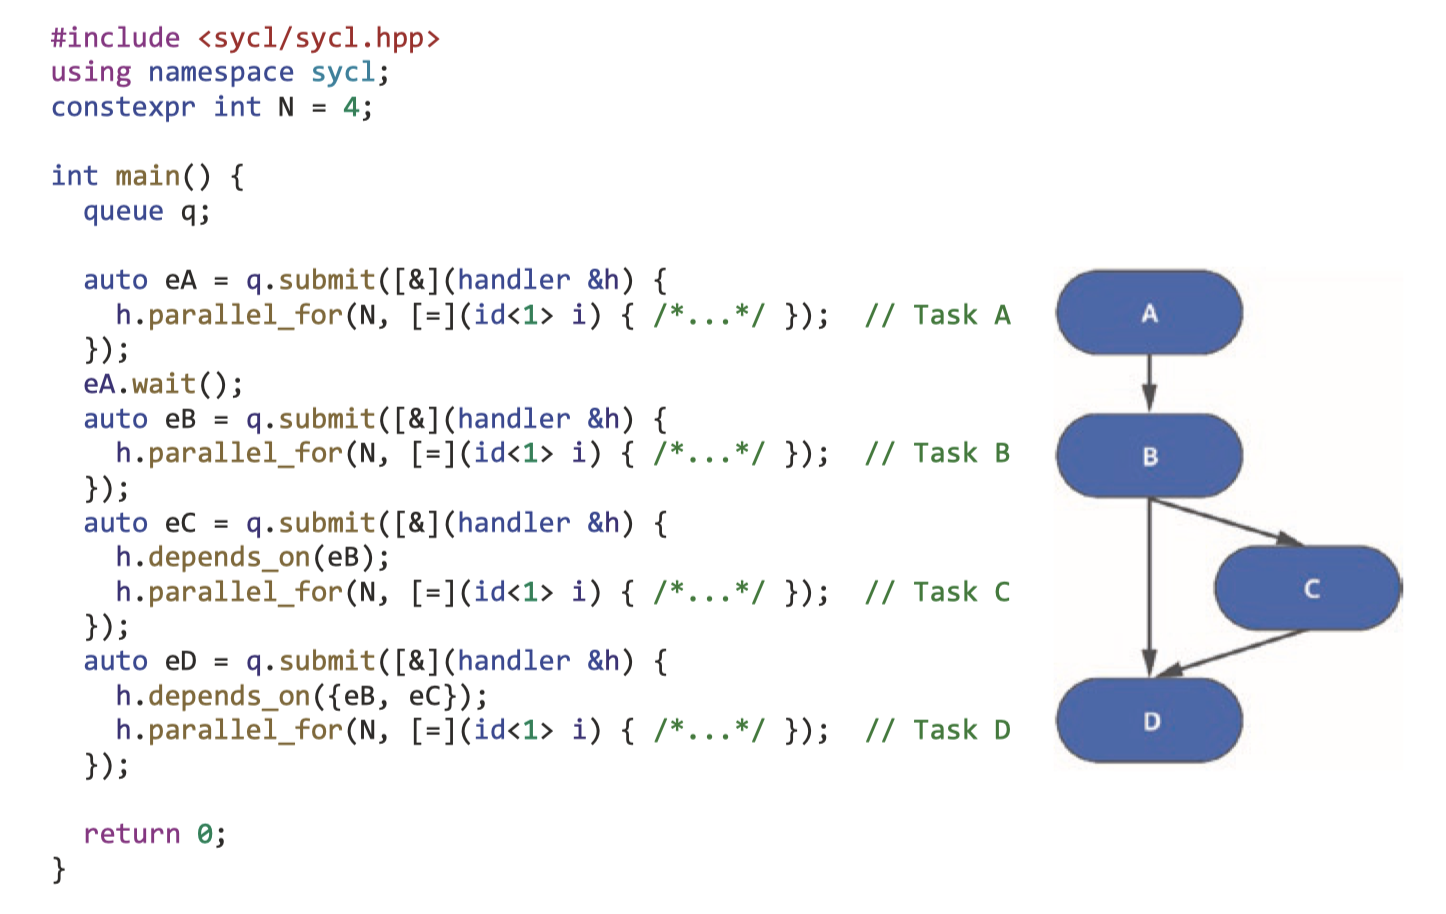
\includegraphics[width=0.9\textwidth]{figs/F3.11.png}
	\caption{\textit{Using events and depends\_on}}
\end{figure}

\paragraph{与访问器的隐式依赖关系}

\begin{figure}[H]
	\centering
	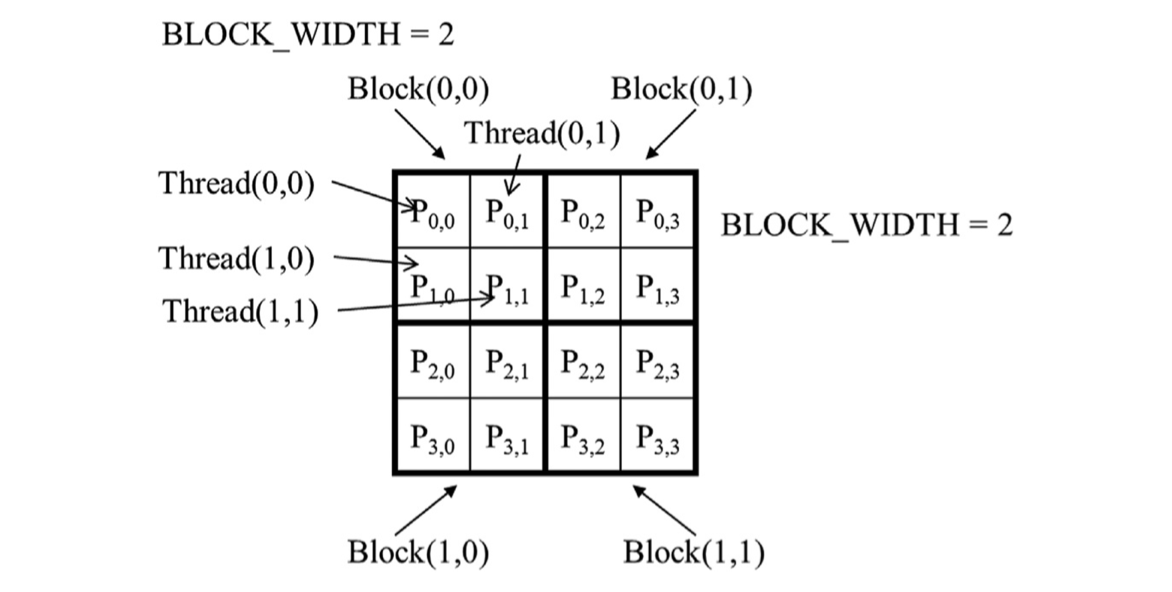
\includegraphics[width=0.9\textwidth]{figs/F3.12.png}
	\caption{\textit{Three forms of data dependences}}
\end{figure}

任务之间的隐式依赖关系是根据数据依赖关系创建的。 任务之间的数据依赖关系有三种形式,如图 3-12 所示。

\begin{figure}[H]
	\centering
	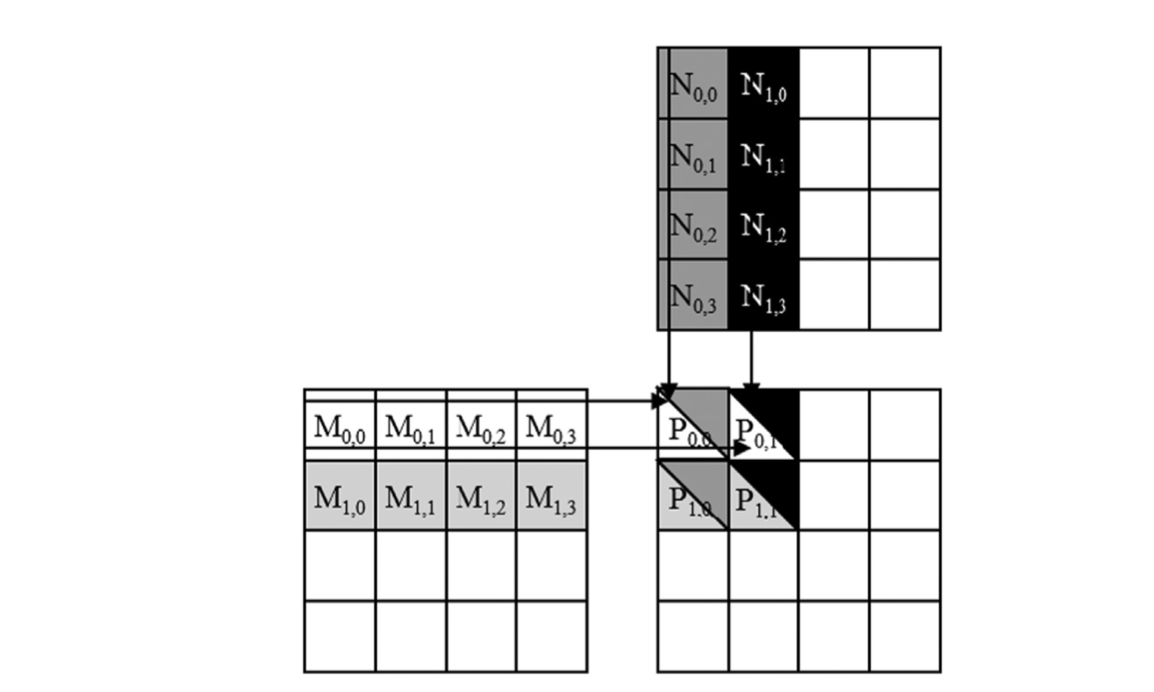
\includegraphics[width=0.9\textwidth]{figs/F3.13.png}
	\caption{\textit{Read-after-Write}}
\end{figure}

\begin{figure}[H]
	\centering
	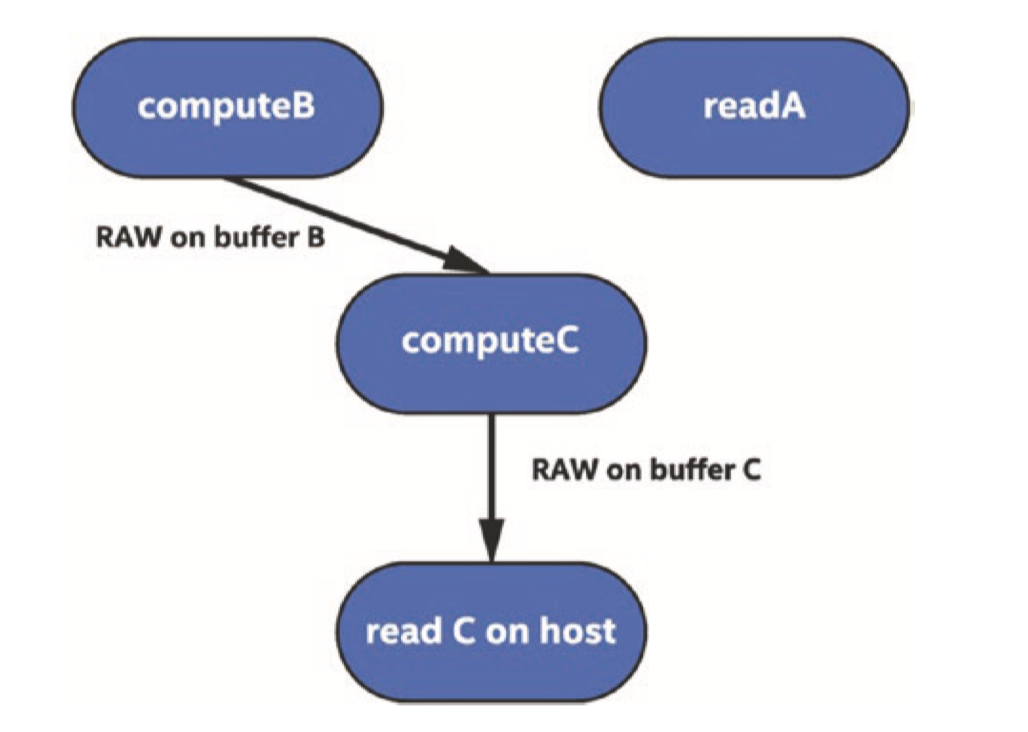
\includegraphics[width=0.9\textwidth]{figs/F3.14.png}
	\caption{\textit{RAW task graph}}
\end{figure}

数据依赖性以两种方式表达给运行时:访问器和程序顺序。 运行时必须使用两者来正确计算数据依赖性。 
图 3-13 和 3-14 对此进行了说明。

在图 3-13 和 3-14 中,我们执行三个Kernel——computeB、readA 和computeC——然后在主机上读回最终结果。 
KernelcomputeB的命令组创建两个访问器a和b。 这些访问器使用访问标记 read\_only 和 write\_only 进行优化,
以指定我们不使用默认访问模式 access\_mode::read\_write。 我们将在第 7 章中了解有关访问标记的更多信息。
KernelcomputeB 读取 Buffer a\_buf 并写入 Buffer b\_buf。 
在Kernel开始执行之前,必须将 Buffer a\_buf 从主机复制到设备。

Kernel readA 还为Buffer a\_buf 创建一个只读访问器。 
由于Kernel readA 是在KernelcomputeB 之后提交的,因此这会创建 Read-afterRead (RAR) 场景。 
然而,RAR 不会对运行时施加额外的限制,并且Kernel可以自由地以任何顺序执行。 
事实上,运行时可能更喜欢在KernelcomputeB之前执行KernelreadA,甚至同时执行两者。 
两者都需要将Buffer a\_buf 复制到设备,但KernelcomputeB还需要复制Buffer b\_buf,
以防任何现有值不被 computeB 覆盖并且可能被以后的Kernel使用。 
这意味着运行时可以在Buffer b\_buf 的数据传输发生时执行Kernel readA,并且还表明即使Kernel仅写入Buffer,
Buffer的原始内容仍可能被移动到设备,
因为无法保证 Buffer中的所有值都将由Kernel写入(请参阅第 7 章了解允许我们在这些情况下进行优化的标签)。

KernelcomputeC读取Buffer b\_buf,这是我们在KernelcomputeB中计算的。 
由于我们在提交KernelcomputeB之后提交了KernelcomputeC,这意味着KernelcomputeC对Buffer b\_buf 有RAW数据依赖。 
RAW 依赖关系也称为真实依赖关系或流依赖关系,因为数据需要从一个计算流到另一个计算才能计算出正确的结果。 
最后,我们还在KernelcomputeC和主机之间创建对Buffer c\_buf 的RAW依赖,因为主机希望在Kernel完成后读取C。 
这会强制运行时将Buffer c\_buf 复制回主机。 
由于设备上没有对Buffer a\_buf 进行写入,因此运行时不需要将该Buffer复制回主机,因为主机已经拥有最新的副本。

\begin{figure}[H]
	\centering
	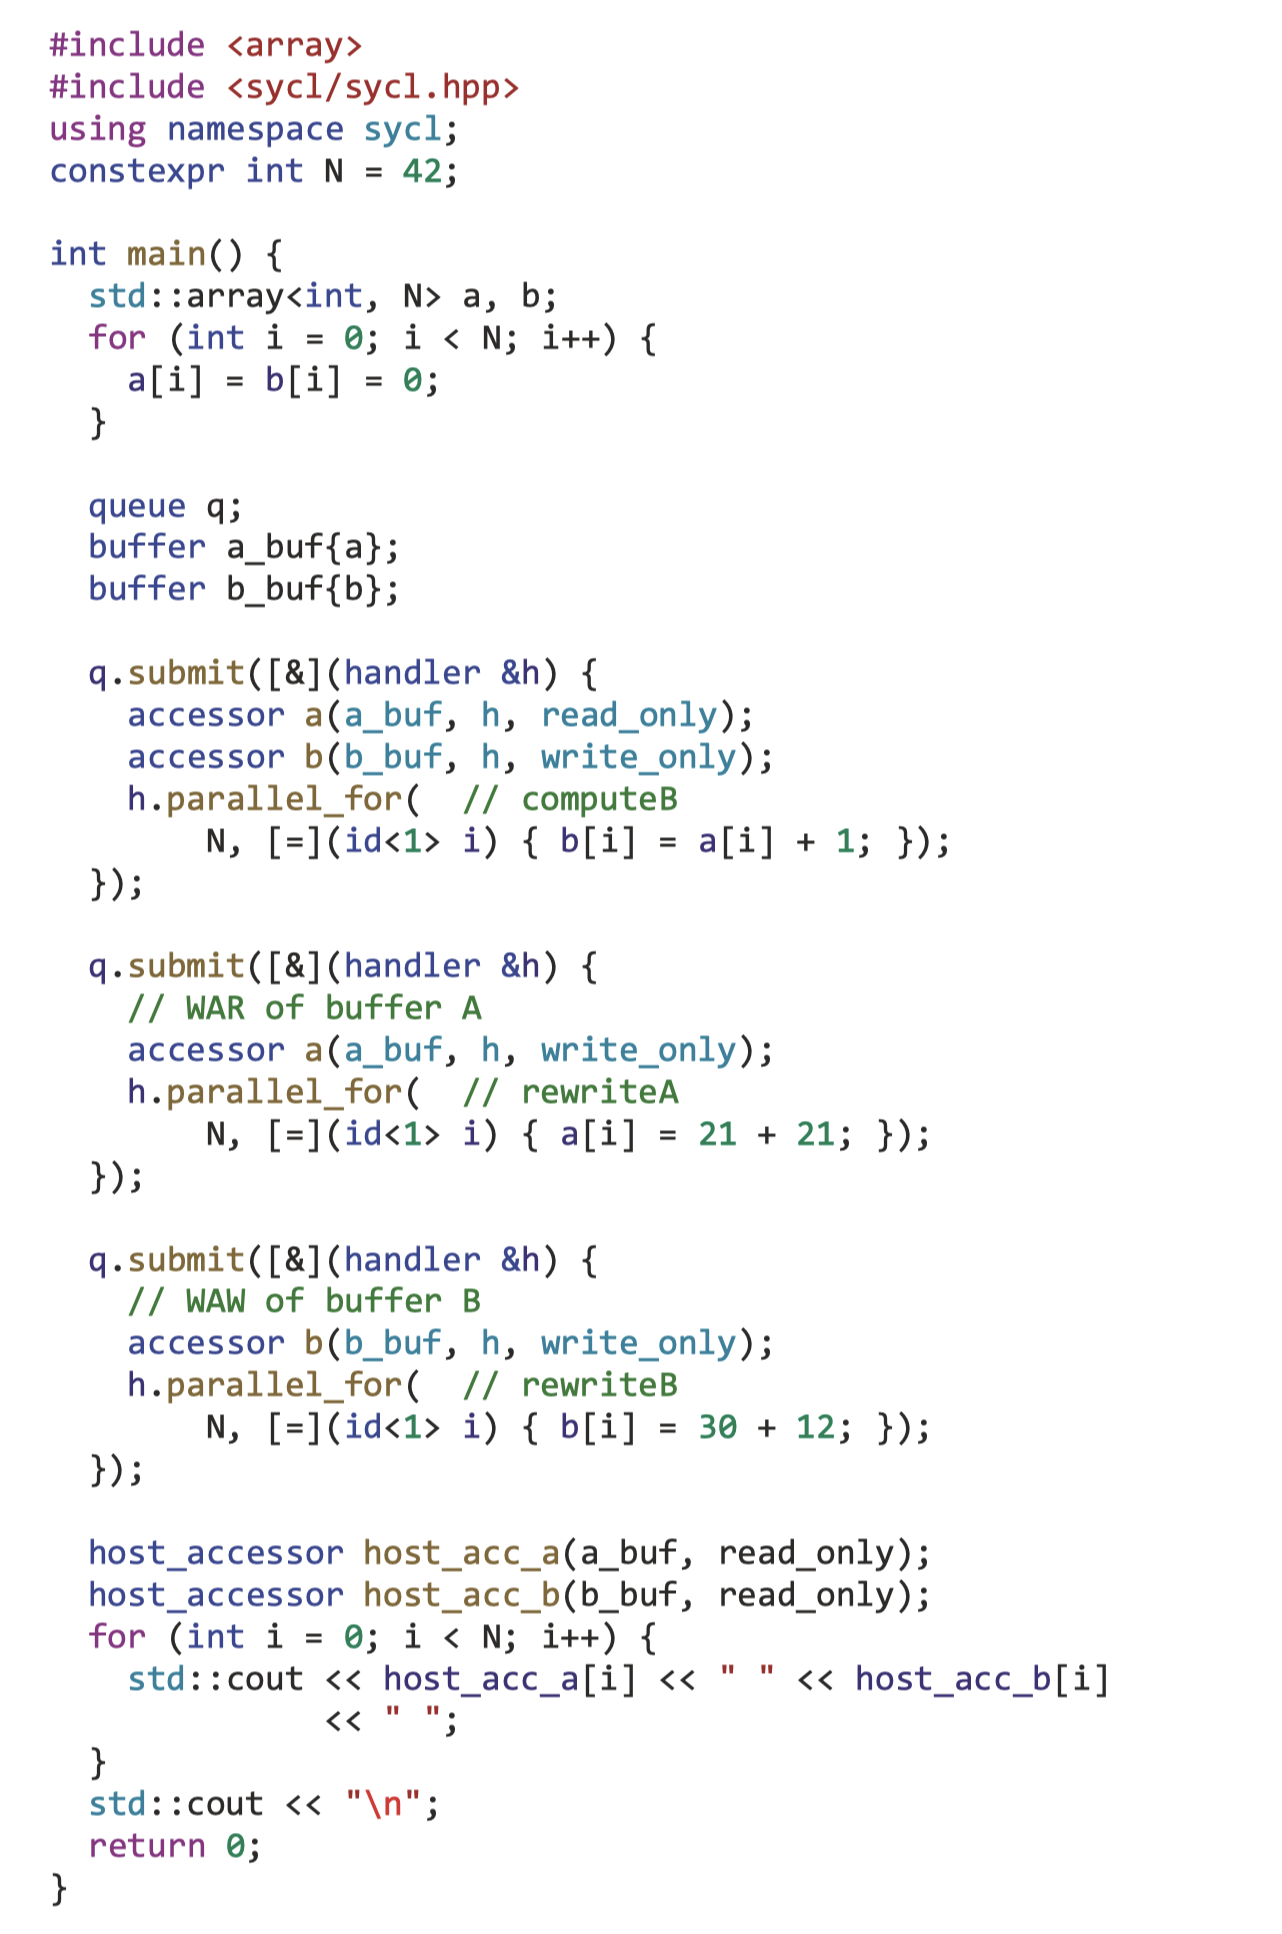
\includegraphics[width=0.9\textwidth]{figs/F3.15.png}
	\caption{\textit{Write-after-Read and Write-after-Write}}
\end{figure}

\begin{figure}[H]
	\centering
	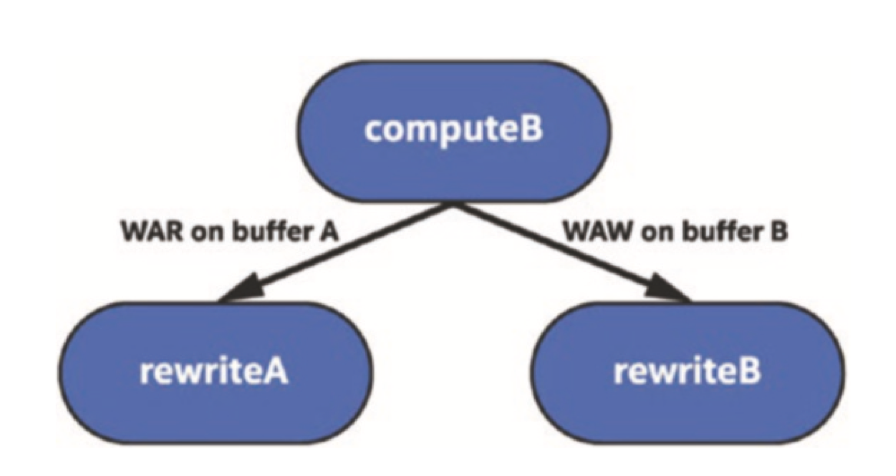
\includegraphics[width=0.9\textwidth]{figs/F3.16.png}
	\caption{\textit{WAR and WAW task graph}}
\end{figure}

在图 3-15 和 3-16 中,我们再次执行三个Kernel:computeB、rewriteA 和 rewriteB。 
KernelcomputeB再次读取Buffer a\_buf 并写入Buffer b\_buf,
KernelrewriteA写入Buffer a\_buf,KernelrewriteB写入Buffer b\_buf。 
理论上,Kernel rewriteA 可以比KernelcomputeB 更早执行,因为在Kernel准备好之前需要传输的数据较少,
但它必须等到KernelcomputeB 完成之后,因为对Buffer a\_buf 存在WAR 依赖性。

在这个例子中,KernelcomputeB需要来自主机的A的原始值,
如果KernelrewriteA在KernelcomputeB之前执行,它将读取错误的值。 
WAR 依赖也称为反依赖。 RAW 依赖性确保数据正确地流向正确的方向,而 WAR 依赖性确保现有值在读取之前不会被覆盖。 
WAW 对Buffer b\_buf 的依赖在Kernel重写函数中也类似。 
如果在KernelcomputeB和rewriteB之间提交了对Buffer b\_buf 的任何读取,它们将导致RAW和WAR依赖性,从而正确排序任务。 
然而,在此示例中,Kernel rewriteB 和主机之间存在隐式依赖性,因为最终数据必须写回主机。 
我们将在第 7 章中详细了解导致此写回的原因。WAW 依赖性,也称为输出依赖性,可确保最终输出在主机上正确。

\subsection{选择数据管理策略}
为我们的应用程序选择正确的数据管理策略很大程度上取决于个人喜好。 
事实上,我们可能会从一种策略开始,随着我们的项目成熟而转向另一种策略。 
然而,有一些有用的指南可以帮助我们选择满足我们需求的策略。

首先要做的决定是我们是否要使用显式或隐式数据移动,因为这极大地影响了我们需要对程序执行的操作。 
隐式数据移动通常是一个更容易开始的地方,因为所有数据移动都为我们处理,让我们专注于计算的表达。

如果我们决定从一开始就完全控制所有数据移动,那么我们要从使用 USM 设备分配的显式数据移动开始。 
我们只需要确保在主机和设备之间添加所有必要的副本即可!

当选择隐式数据移动策略时,我们仍然可以选择是使用Buffer还是USM主机或共享指针。 
同样,这种选择取决于个人喜好,但有几个问题可以帮助我们选择其中一个。 
如果我们要移植使用指针的现有 C/C++ 程序,USM 可能是一条更简单的路径,因为大多数代码不需要更改。 
如果数据表示没有引导我们做出偏好,我们可以问的另一个问题是我们希望如何表达Kernel之间的依赖关系。 
如果我们更愿意考虑Kernel之间的数据依赖性,请选择Buffer。 
如果我们更愿意将依赖关系视为在另一项计算之前执行一项计算,
并希望使用有序队列或显式事件或Kernel之间的等待来表达这一点,请选择 USM。

当使用 USM 指针(显式或隐式数据移动)时,我们可以选择要使用哪种类型的队列。 
有序队列简单直观,但它们限制了运行时间并可能限制性能。 
无序队列更复杂,但它们为运行时提供了更大的自由度来重新排序和重叠执行。 
如果我们的程序在Kernel之间具有复杂的依赖关系,那么无序队列类是正确的选择。 
如果我们的程序只是一个接一个地运行许多Kernel,那么有序队列对我们来说将是一个更好的选择。

\subsection{Handler类:关键成员}
\begin{figure}[H]
	\centering
	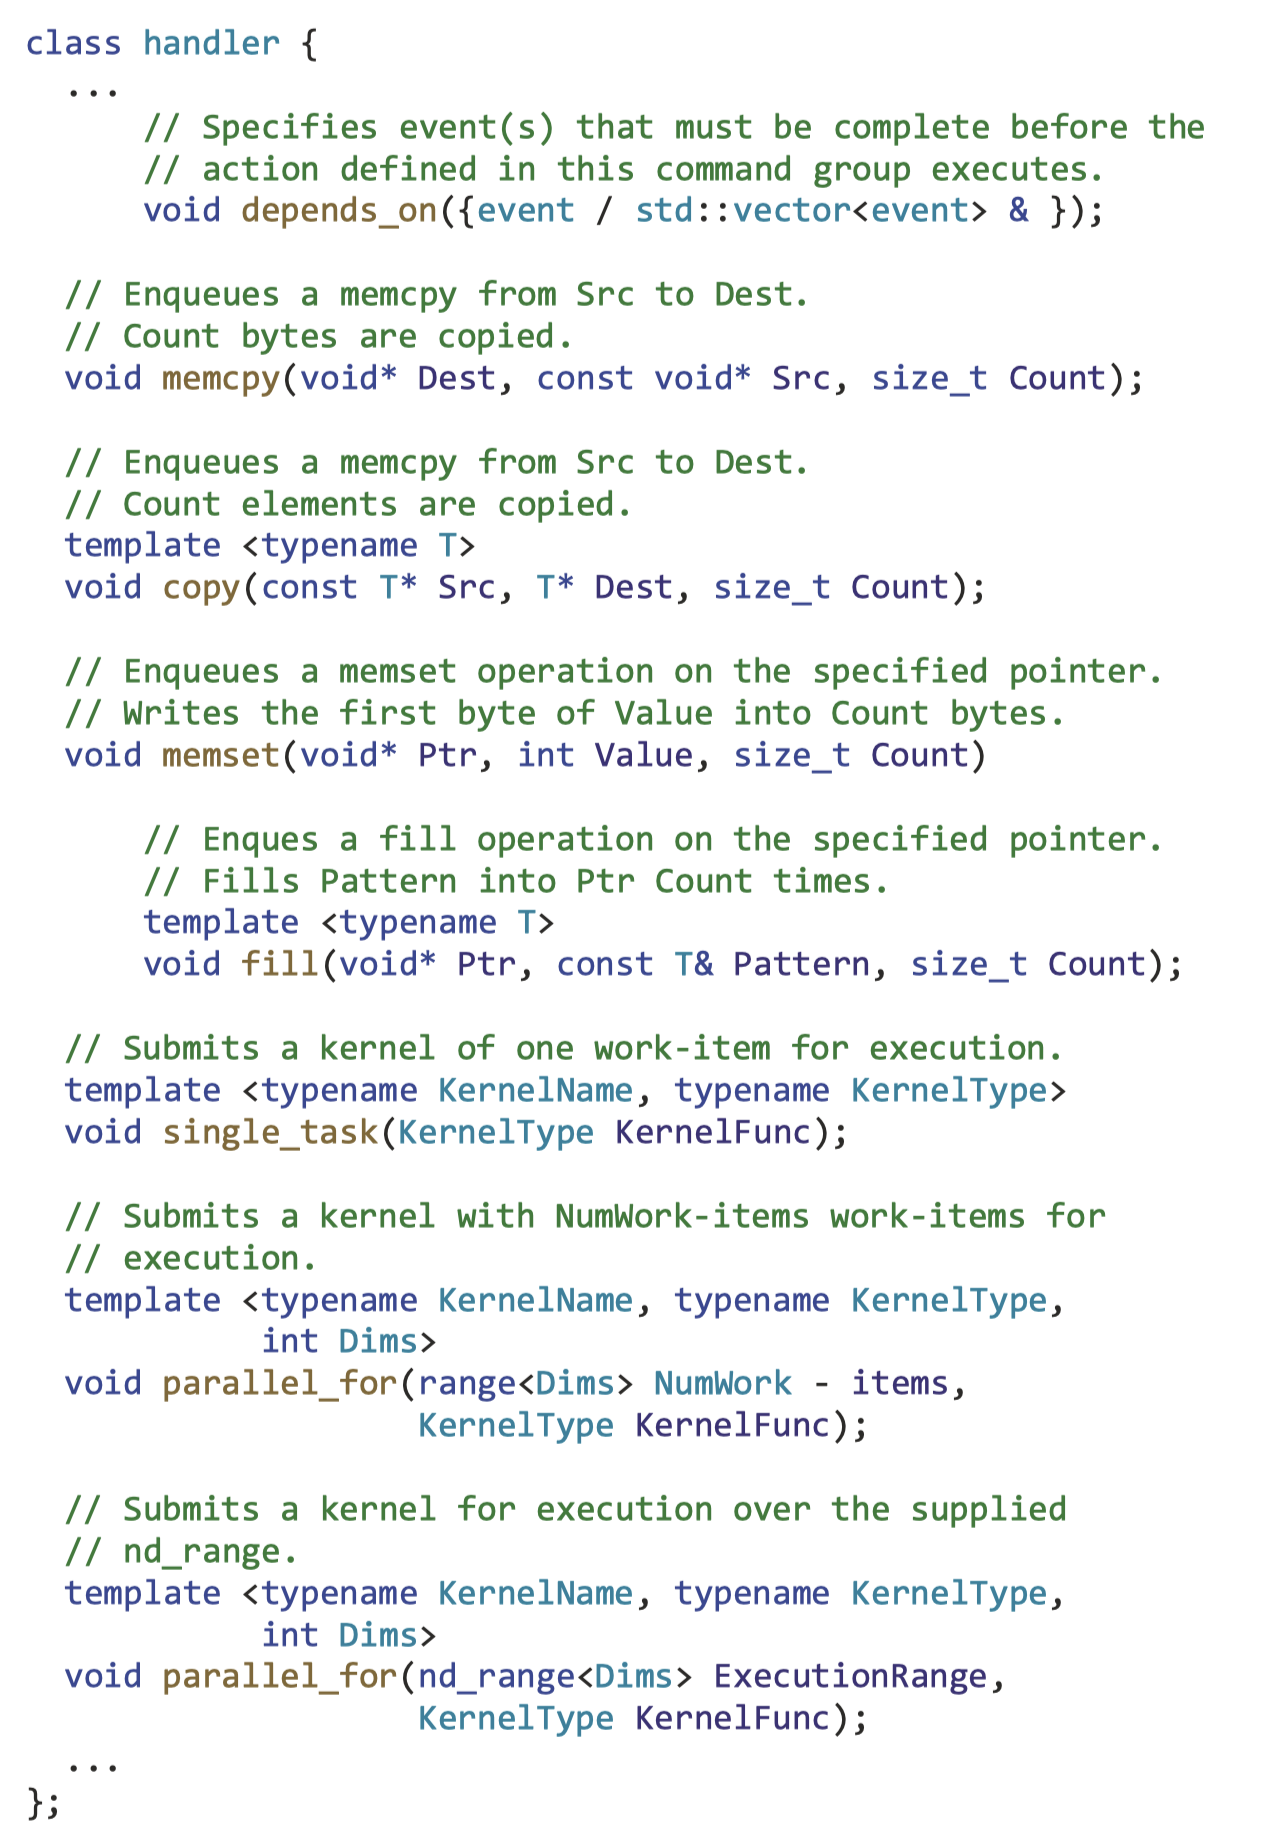
\includegraphics[width=0.9\textwidth]{figs/F3.17.png}
	\caption{\textit{Simplified definition of the non-accessor members of the handler class}}
\end{figure}

\begin{figure}[H]
	\centering
	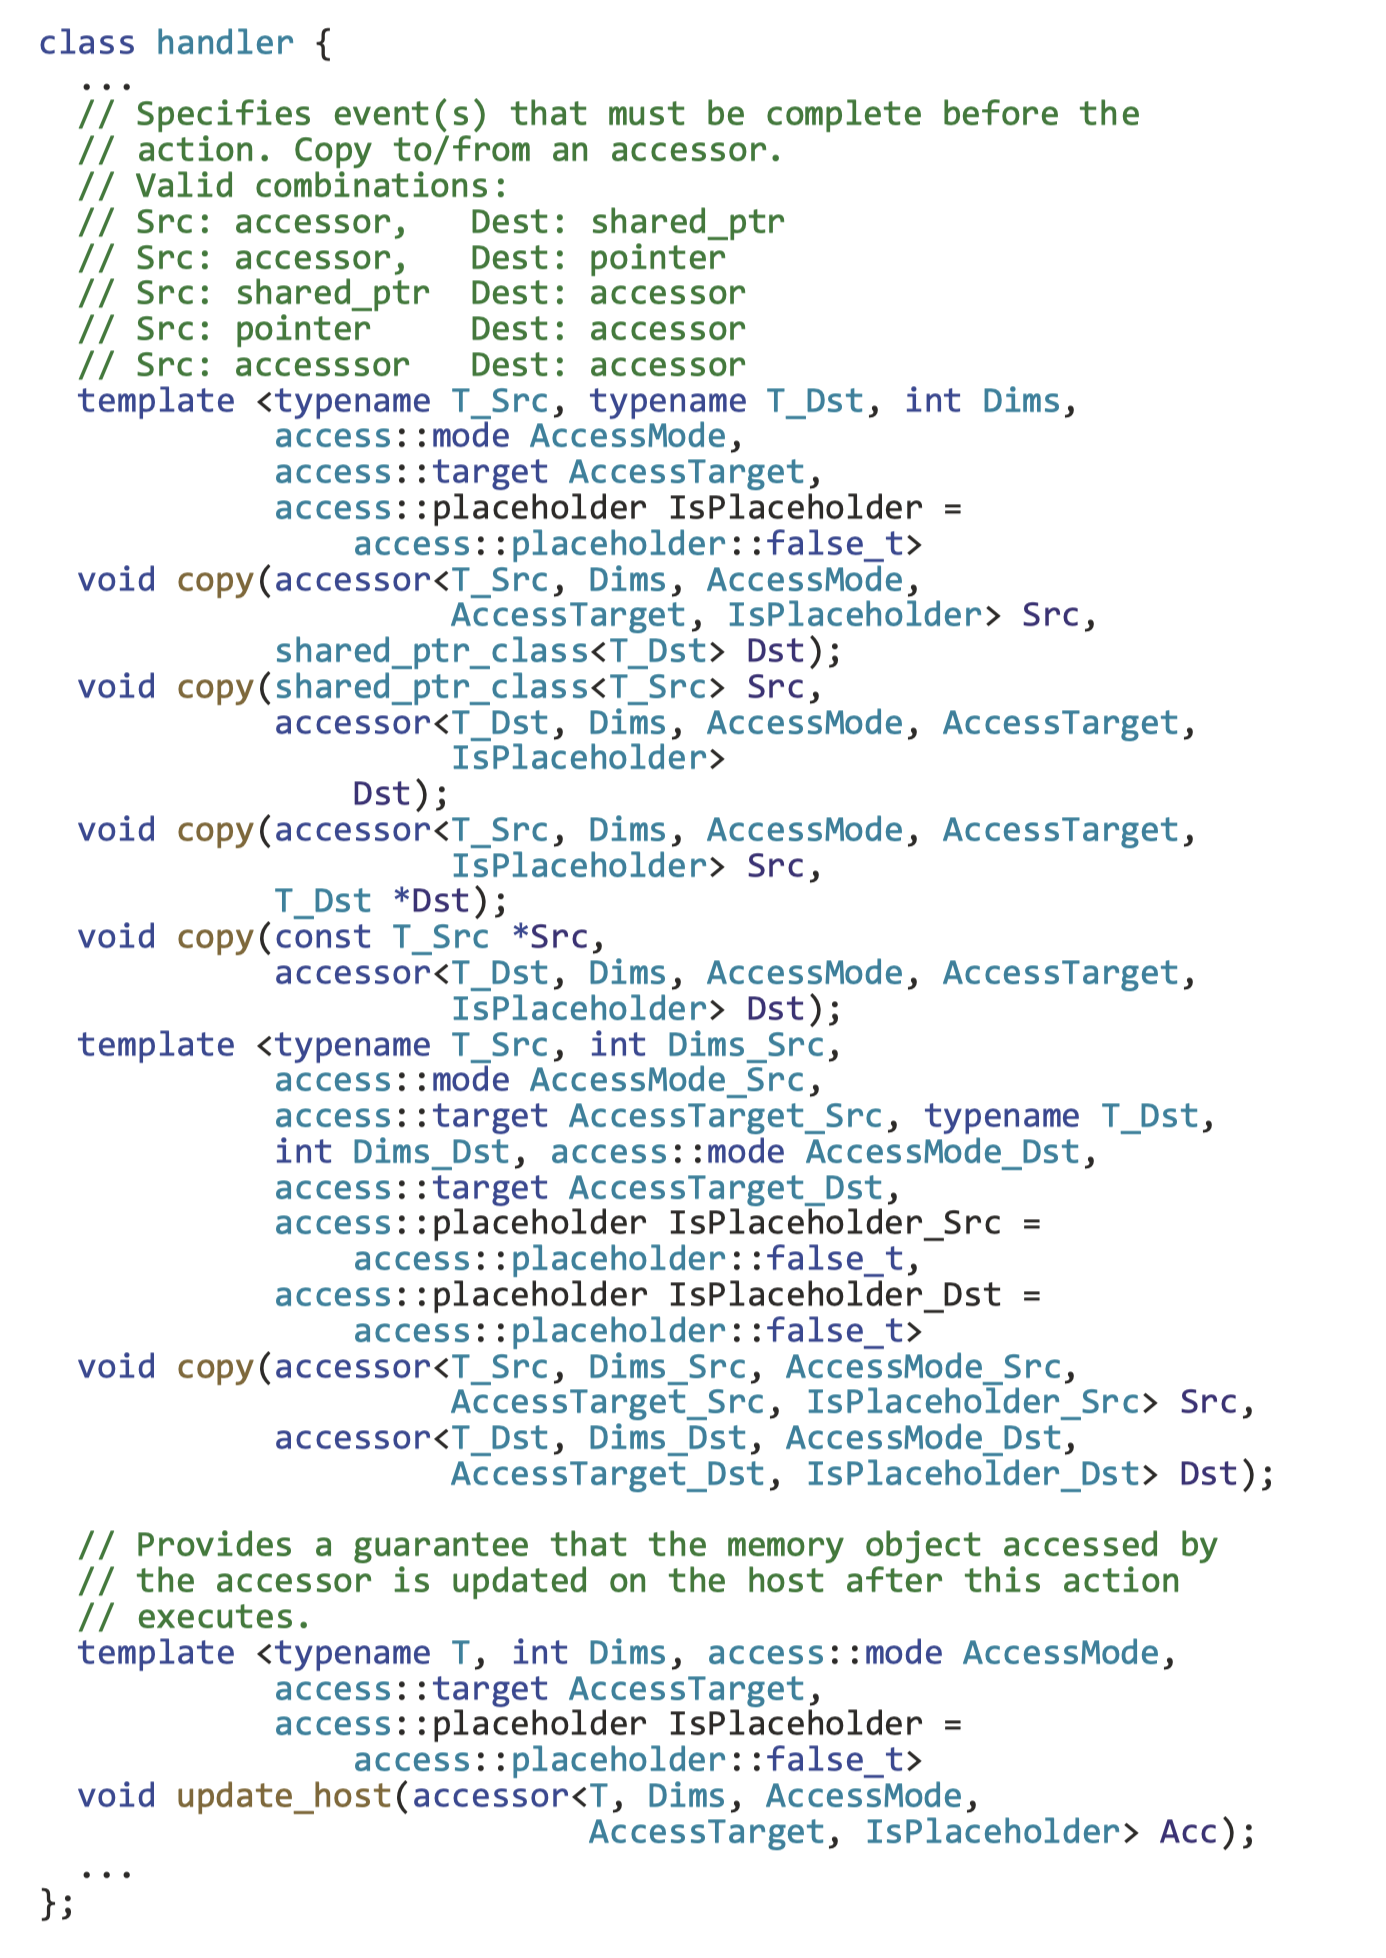
\includegraphics[width=0.9\textwidth]{figs/F3.18.png}
	\caption{\textit{Simplified definition of the accessor members of the handler class}}
\end{figure}

我们已经展示了多种使用Handler类的方法。 图 3-17 和 3-18 提供了这个非常重要的类的关键成员的更详细的解释。 
我们还没有使用所有这些成员,但稍后将在本书中使用它们。 这是放置它们的好地方。

一个密切相关的类,队列类,在第 2 章末尾有类似的解释。

\subsection{总结}
在本章中,我们介绍了解决数据管理问题的机制以及如何排序数据的使用。 
使用加速器设备时,管理对不同内存的访问是一个关键挑战,我们有不同的选项来满足我们的需求。

我们概述了数据使用之间可能存在的不同类型的依赖关系,
并描述了如何向队列提供有关这些依赖关系的信息,以便它们正确排序任务。

本章概述了统一共享内存和Buffer。 我们在第 6 章中更详细地探讨了 USM 的所有模式和行为。
第 7 章更深入地探讨了Buffer,包括创建Buffer和控制其行为的所有不同方法。 
第 8 章回顾了控制Kernel执行和数据移动顺序的队列调度机制。